\section{Exploring Thread Interleaving Space}
\label{s:design}

\newcommand{\intcov}{interleaving segment coverage\xspace}
\newcommand{\Intcov}{Interleaving segment coverage\xspace}


% In this section, we describe our approach to effectively achieve
% \textbf{Design goal 1} and \textbf{2}.


%
% Specifically, we propose a novel perspective on the thread
% interleaving exploration.
% %
% Specifically, our key idea lies in three steps:

This work focuses on how to efficiently explore the large search space
of thread interleaving when a multi-thread input (\eg,
\texttt{sendmsg()} and \texttt{setsockopt()} in
\autoref{fig:cve-2017-17712}) is given. Our approach utilizes an
\textit{explored} thread interleaving as a seed interleaving.
%
With the seed interleaving, we explore thread interleavings of 
a given multi-thread input in the following three steps:
%
\begin{enumerate}[labelsep=0pt, label=\textbf{\arabic*) }]
\item \textbf{\textit{Decomposing}} an explored thread interleaving
  into segments containing a small number of instructions.
\item \textbf{\textit{Mutating}} interleavings within a segment to
  generate unexplored interleavings for each segment.
\item \textbf{\textit{Recomposing}} mutated segments into whole thread
  interleaving to determine how to schedule instructions.\yj{revisit
    this sentence}.
\end{enumerate}
%



In this section, we first explain our key intuition behind
decomposing a thread interleaving into \textit{interleaving
  segments}~(\autoref{ss:overview}).
%
Then, we illustrate how we define an interleaving coverage metric 
from decomposed interleaving segments.
%
% The coverage metric represents
% combinatorial interleavings\yj{I do not like the term, combinatorial interleaving. Is it widely used?} (\textbf{Design goal
%   1})~(\autoref{ss:coverage}).
%
Lastly, we explain the speculative interleaving exploration method,
which speculates whole interleaving based on mutated segments to guide
instruction scheduling ~(\textbf{Design goal
  2})~(\autoref{ss:scheduler}). \yj{a new thread?}
% interleaving for future iterations (\textbf{Design goal
%   2})~(\autoref{ss:scheduler}).



\subsection{Key Idea: Segmentizing thread interleaving}
\label{ss:overview}

%\begin{table}[t]
  %\centering
  %input{table/learningfrommistakes.tex}
  %\caption{Statistics provided by Shan Lu
    %\etal~\cite{learningfrommistakes}, stating the number of
    %concurrency bugs according to the number of memory accesses
    %involved in the manifestation of a concurrency bug. \yj{Do we need
      %the table?} \dr{No. we can remove this.}}
  %\label{table:learningfrommistakes}
  % \end{table}

When fuzzing for discovering concurrency bugs with a coverage metric,
the fundamental challenge is the large search space because
combinations of thread interleavings increase the search space
exponentially.
%
Therefore, this work seeks to strike the balance in the trade-off
between the bug-finding capability and the search complexity.

\PP{Segmentizing thread interleaving}
%
To reduce the search complexity, we take the classical wisdom of
problem decomposition where the complexity of a problem exponentially
decreases as the problem size decreases.
%
Our key strategy is \textit{decomposing} the search space into small
sub-spaces. We call a sub-space \textit{interleaving segment}.
%
Each interleaving segment consists of instructions accessing 
shared memory objects.
% the same  memory objects. (\ie, conflicting instructions).
To define the size (the number of instructions) of an interleaving segment,
we use an observation from a previous study~\cite{learningfrommistakes} 
in which 92.4\% (97 out of 105) of concurrency bugs manifest when a bug-finding system
monitors specific interleaving orders of \textit{at most} four memory
accesses referring to shared memory objects.
%
So, all other memory accesses beyond four accesses and their execution
orders do not meaningfully affect manifestation of a concurrency bug.
%
The observation is also applied to the example of
\autoref{fig:cve-2017-17712}. The uninitialized access bug is
triggered by the execution order of three memory accesses (\eg,
\texttt{A2}, \texttt{A4} and \texttt{B1}), while others (\eg,
\texttt{A6} and \texttt{B2}) are irrelevant to the manifestation of
the concurrency bug.
Following the observation,  we confine the size of a interleaving segment 
to contain at most four memory-accessing instructions,
which makes the problem of defining a coverage metric tractable while maintaining a strong bug-finding capability.


\PP{Example of interleaving segments}
%
\begin{figure}[t]
  \centering
  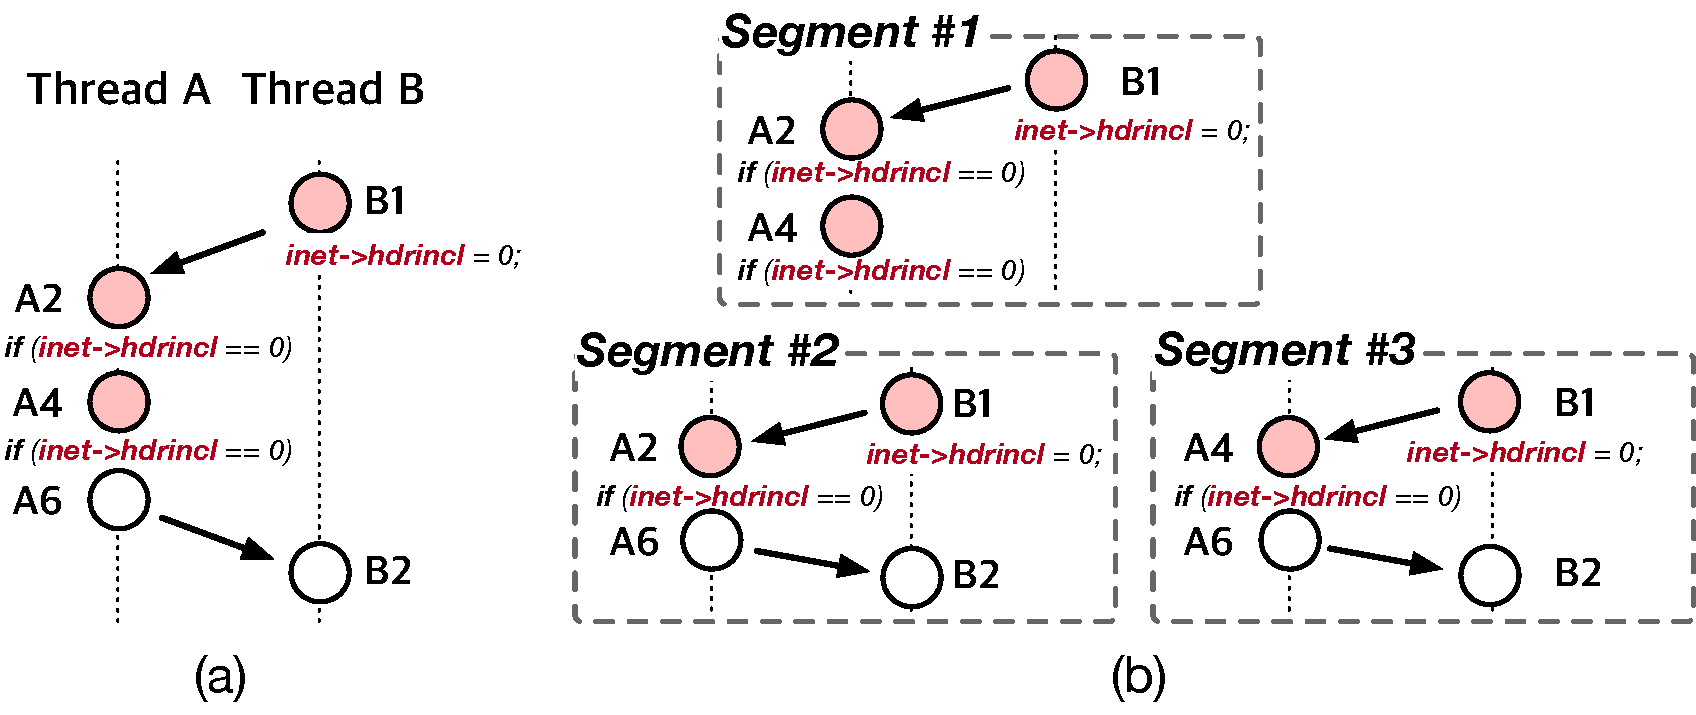
\includegraphics[width=0.99\linewidth]{fig/intuition.pdf}
  \caption{(a) A thread interleaving example of
    \autoref{fig:cve-2017-17712}, and (b) interleaving segments
    contained in (a).  Note that we intentionally omit instructions
    that do not access globally-visible memory objects.}
  \label{fig:keyidea}
\end{figure}
%
\yj{interleaving vs interleavings?}
\autoref{fig:keyidea} illustrates three interleaving segments 
from the single execution of two system calls, 
%thread interleaving.
%
where the execution scenario is represented in
\autoref{fig:keyidea}-(a).
% example shows the execution of the two system calls 
% and executed thread interleavings described in
%
Then, interleaving segments described in \autoref{fig:keyidea}-(b)
represents a part of its thread interleaving, comprised by at most
four instructions.
%
For example, \texttt{Segment \#1} represents interleavings of three
instructions \texttt{B1}, \texttt{A2}, and \texttt{A4}, stating that
\texttt{B1} is executed before \texttt{A2} and \texttt{A4}.
%
Similarly, \texttt{Segment \#2} and \texttt{Segment \#3} describe
interleavings of (\texttt{B1}, \texttt{A2}, \texttt{A6}, and
\texttt{B2}), and (\texttt{B1}, \texttt{A4}, \texttt{A6}, and
\texttt{B2}) respectively.
How to build segments is described in \autoref{ss:coverage}.

%
%Accordingly, a fuzzer can decide that it is worth investing more
%computing power to further explore thread interleavings.
%
%Moreover, a fuzzer can infer exact execution orders that have not been
%explored, 
%
%A fuzzer therefore can systematically search thread interleavings
%directed by the inference, rather than random searching.


% Segmentizing this thread interleaving is performed in two steps.
% %
% First, we pair up two instructions that access the same mermoy object.
% %
% In \autoref{fig:keyidea}-(a), there are three pairs of such
% interleaved instructions such as
% ($\texttt{B1} \Rightarrow \texttt{A2}$) and
% ($\texttt{B1} \Rightarrow \texttt{A4}$) (accessing
% \texttt{inet->hdrincl}), and ($\texttt{A6} \Rightarrow \texttt{B2}$)
% (accessing \texttt{sk->owned}).
% %
% As we want to represent a combination of interleaving orders, the
% second step is to further combine instruction pairs into an
% interleaving segment.
% %
% Each interleaving segment is formed by combining two instruction pairs
% so that interleaving segments contain at most four instructions.
% %
% For example, we combine two instruction pairs
% ($\texttt{B1} \Rightarrow \texttt{A2}$) and
% ($\texttt{B1} \Rightarrow \texttt{A4}$) to construct \texttt{Segment
%   \#1} in which three instructions \texttt{B1}, \texttt{A2}, and
% \texttt{A4} are included.
% %
% In accordance with timestamps annotated in these instructions, we can
% arrange the instructions in \texttt{Segment \#1}.
% %
% Likewise, \texttt{Segment \#2} and \texttt{Segment \#3} are the result
% of combining $\texttt{B1} \Rightarrow \texttt{A2}$ and
% $\texttt{A6} \Rightarrow \texttt{B2}$, and
% $\texttt{B1} \Rightarrow \texttt{A4}$ and
% $\texttt{A6} \Rightarrow \texttt{B2}$ respectively.

%
% \autoref{fig:keyidea}-(a) represents the thread interleaving of the
% execution, where the uninitialized access bug does not manifest
% because \texttt{B1} is executed before \texttt{A4} (\ie,
% $(\texttt{A2} \Rightarrow \texttt{B1}) \wedge (\texttt{B1} \Rightarrow
% \texttt{A4})$ is not satisfied).
% %
% In order to track interleaving orders of a small number (\eg, four) of
% instructions, we decompose the thread interleaving into several
% interleaving segments as described in \autoref{fig:keyidea}-(b).
% %
% In these interleaving segments, \texttt{Segment \#1} contains three
% memory access operations (\ie, \texttt{A2}, \texttt{A4}, and
% \texttt{B1}), and describes interleaving orders such that \texttt{B1}
% is executed after \texttt{A2} and \texttt{A4}.
% %
% Similarly, \texttt{Segment \#2} and \texttt{Segment \#3} describes
% interleaving orders of four memory access operations, (\texttt{A2},
% \texttt{B1}, \texttt{B2}, \texttt{A6}) and (\texttt{A4}, \texttt{B1},
% \texttt{B2}, \texttt{A6}) respectively.
%

% With these interleaving segments, the fuzzer can be noticed that
% interleaving orders represented by these interelaving segments
% unlikley cause a concurrency bug.
% %
% Therefore, it is adequate for the fuzzer to search for unexplored
% interleaving segments (\eg, one that represents
% $(\texttt{A2} \Rightarrow \texttt{B1}) \wedge (\texttt{B1} \Rightarrow
% \texttt{A4})$) to maximize the chance of discovering concurrency bugs.


% %
% \dr{}
% It is worth noting that interleaving segments can be overlapped; in
% this example, \texttt{Segment \#1} and \texttt{Segment \#3} are
% overlapped over an interleaving order
% $\texttt{A4} \Rightarrow \texttt{B1}$.




\PP{Benefits of segmentizing thread interleaving}
%
Segmentizing instruction interleavings provides two 
benefits to a fuzzer.
%
First, when defining a coverage metric, tracking explored interleavings
in each segment gives a befitting guidance to determine whether a 
fuzzer further explores thread interleavings or not. 
%
% As mentioned above, most concurrency bugs manifest depending only on
% the execution order of four memory accesses.
%
Considering most concurrency bugs manifest depending on interleaving
orders of at most four memory accesses (which is exactly represented
by an interleaving segment), 
if a fuzzer explores all possible interleavings for each detected segment,
it is unlikely that a fuzzer misses a concurrency bug.
%
Accordingly, \textit{interleaving orders in each segment can act as an
interleaving coverage metric, satisfying \textbf{Design goal 1}}.


% \Intcov and the form of segment graph express semantically rich
% information; it captures combinations of multiple pairs of interleaved
% instructions. At the same time, segment graphs are represented simply;
% each segment graph contains only at most four instructions.

% These two seemingly-conflicting characteristics of segment graphs
% enables the systematic exploration of thread interleaving.
% %
% In other words, it is practically impossible to thoroughly explore all
% thread interleavings of a given multi-thread input because of the
% astronomical number of possible thread interleavings.
% %
% However, it is \textit{easily possible} to throughly explore
% interleavings \textit{inside} interleaving segments due to their small
% size. More importantly, exploring inside interleaving segments is
% still enough to discover most concurrency bugs (as mentioned in
% \autoref{ss:overview}).




Second, explored interleaving segments can be used to
systematically search for instruction interleavings in next 
iterations.
%
Since each interleaving segment contains only a small number of memory
accesses, a fuzzer can speculatively creates new interleavings
from an explored interleavings.
Taking an example of \texttt{Segment \#1} in \autoref{fig:keyidea},
besides execution order
($\texttt{B1} \Rightarrow \texttt{A2} \Rightarrow \texttt{A4}$)
(represented in \texttt{Segment \#1}), a fuzzer easily rearranges
interleaving orders of the three instructions to speculate 
unexplored execution orders of these instructions such as
$\texttt{A2} \Rightarrow \texttt{B1} \Rightarrow \texttt{A4}$ which
causes the uninitialized access bug if executed.
Therefore, instead of doing a randomized search (in most previous approaches), if a fuzzer figures out which of the enumerated interleavings have not been explored, \textit{a fuzzer can strategically 
explore the search space with speculative interleavings, 
satisfying \textbf{Design goal 2}}.


% 
% \autoref{fig:hint} demonstrates how explored interleaving segments
% can be helpful for future iterations.
% %
% As illustrated in \autoref{fig:hint}, the fuzzer can derive
% \textit{unexplored} \texttt{Segment \#1*} by changing the execution
% order of \texttt{A4} and \texttt{B4} in \textit{explored}
% \texttt{Segment \#1}.
% %
% Since \texttt{Segment \#1*} satisfies
% $(\texttt{A2} \Rightarrow \texttt{B1}) \wedge (\texttt{B1} \Rightarrow
% \texttt{A4})$, the fuzzer can discover the uninitialized access bug if
% it executes thread interleaving containing \texttt{Segment \#1*}.
% %
% In addition, the fuzzer can explore multiple interleaving segments at
% a time.
% %
% Besides \texttt{Segment \#1*}, \texttt{Segment \#3*} can also be
% derived from \texttt{Segment \#3}.
% %
% Interestingly, \texttt{Segment \#1*} and \texttt{Segment \#3*} can be
% used to compose a new thread interleaving.
% %
% By executing a thread interleaving including the two derived
% interleaving segments, the fuzzer is able to quickly test a number of
% interleaving segments.
% %
% In this way, \textit{our proposed scheduler mechanism is designed to
%   quickly explore unexplored interleaving segments, and to satisfy
%   \textbf{R2}}.
% %
% \begin{figure}[t]
%   \centering
%   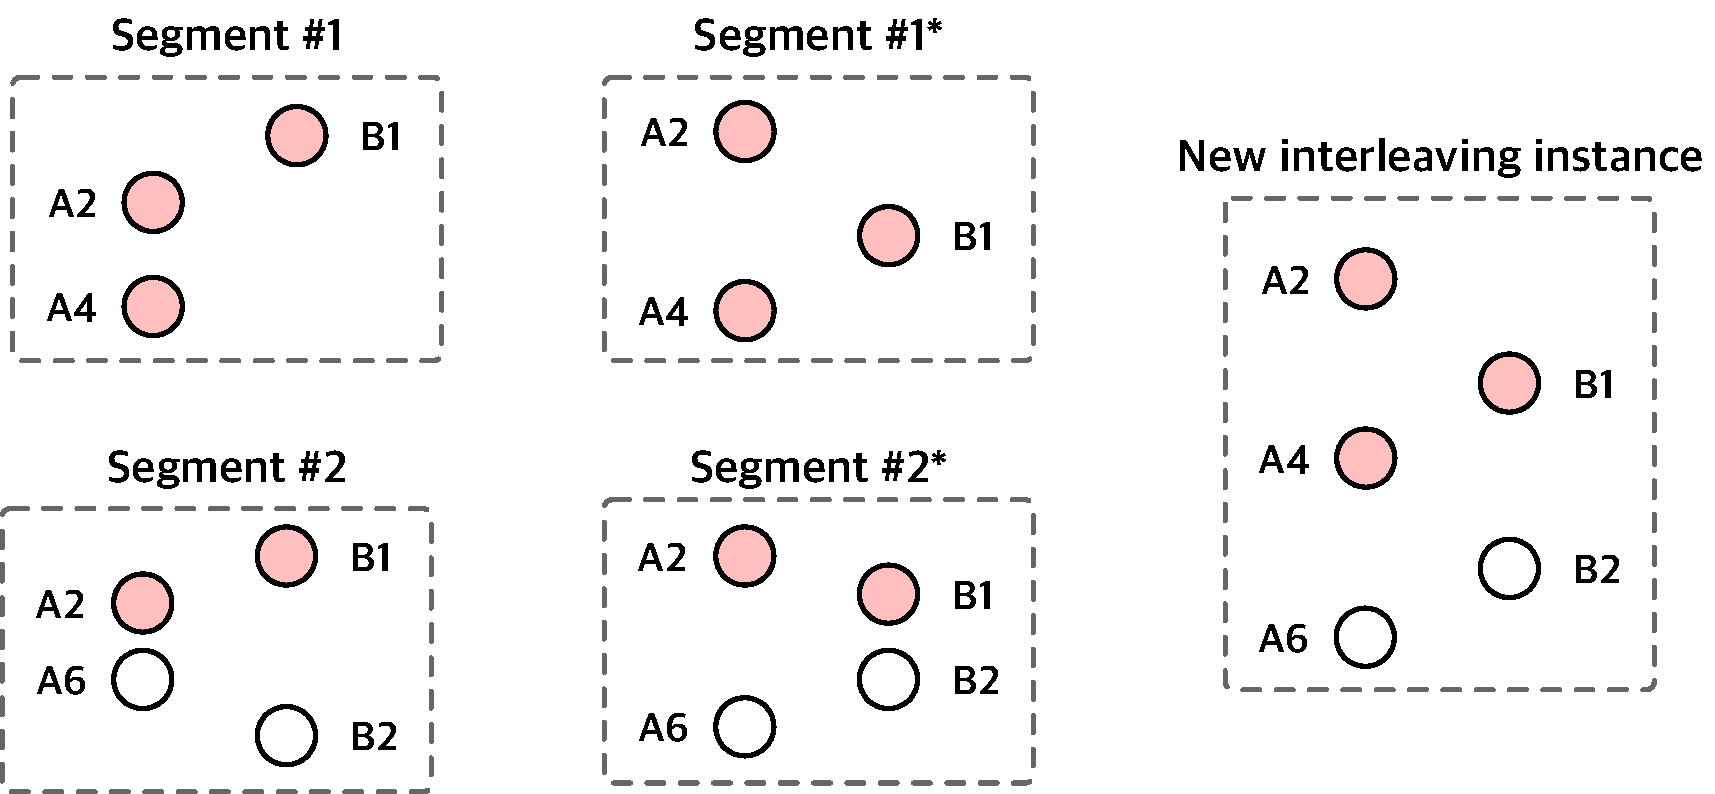
\includegraphics[width=0.9\linewidth]{fig/hint.pdf}
%   \caption{\texttt{Segment \#1} and \texttt{Segment \#3} are explored
%     interleaving segments in \autoref{fig:keyidea}.
%     %
%     From these two interleaving segments, our approach derives other
%     interleaving segments \texttt{Segment \#1*} and \texttt{\#3*}, and
%     schedules instructions to test the derived interleaving segments
%     at the same time.}
%   \label{fig:hint}
% \end{figure}
% %



\subsection{Interleaving Segment Coverage}
\label{ss:coverage}

As discussed, we \textbf{decompose} an explored instruction interleavings
into interleaving segments.
%
We first represent observed interleavings as a directed acyclic graph
(DAG). Then, we compute subgraphs of the DAG called \textit{segment
  graphs}, each of which represents an interleaving segment.



Using a set of segment graphs, we propose a novel interleaving
coverage metric called \textit{\intcov}.
%
\Intcov is a collection of explored segment graphs, designed to track
combinatorial interleaving orders within an interleaving segment.
% , and
% to guide a fuzzer to efficiently search possible instruction
% interleavings.




% Semantically, if
% per-input \intcov is saturated, a fuzzer can confidently conclude that
% the current input unlikely causes a concurrency bug and proceed to the
% next input.
%




\PP{Graph representation of thread interleaving}
% \PP{Graph representation of interleaved instructions}
% As discussed,
% \intcov contains multiple interleaved instructions, 
% so
% \intcov cannot be presented as a single instruction interleaving 
% (e.g., $I_x \rightarrow I_y$) used in the alias coverage used in KRace.
% Instead,
We represent a thread interleaving as a DAG, where
% called an interleaving segment graph (shortly, \textit{segment
%   graph}).
%
a vertex represents a memory-accessing instruction, and an edge
represents an execution ordering between two memory-accessing
instructions. There are two types of edges,
program-order edges and interleaving-order edges.
%
A program-order edge indicates an execution order between two
memory-accessing instruction in a single thread.  Whereas, an
interleaving-order edge indicates the execution order between two
memory-accessing instructions that 1) access the same shared data, 2)
at least one of them is a write operation, and 3) are executed by
different threads.

\begin{figure}[t]
  \centering
  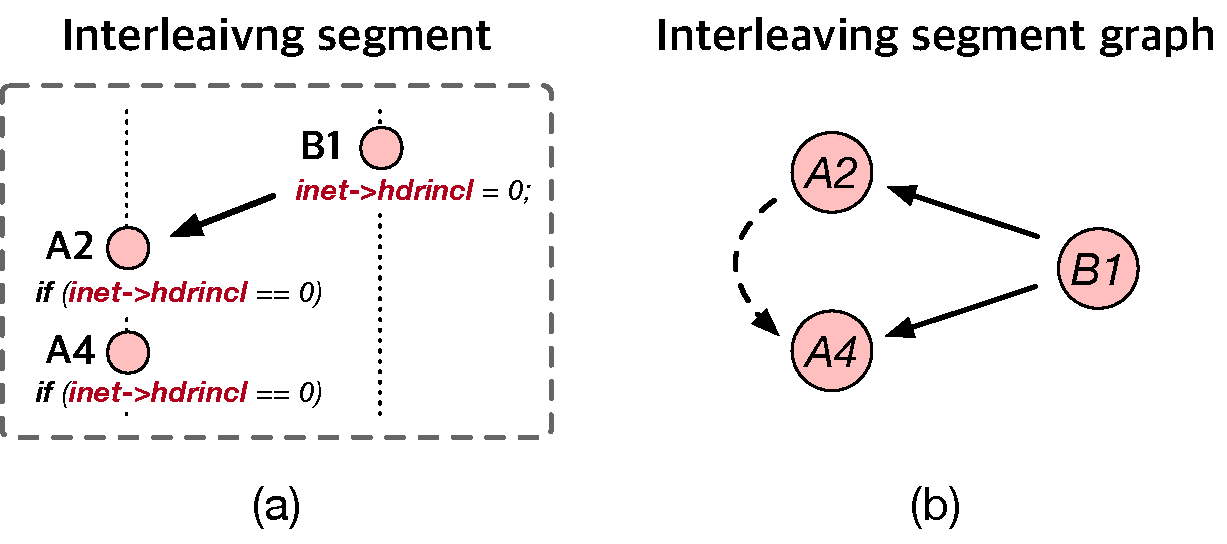
\includegraphics[width=0.8\linewidth]{fig/interleavingsegmentgraph.pdf}
  \caption{(a) Graph representation of \autoref{fig:keyidea}-(a), and
    (b) segment graph corresponding \texttt{Segment \#1} in
    \autoref{fig:keyidea}-(b). In each graph, a dotted arrow
    represents a program-order edge, and solid arrows represent
    interleaving-order edges.}
  \label{fig:interleavingsegmentgraph}
\end{figure}

%It is worth noting that a segmentgraph has two properties. First, if
%a path exists from a vertex \texttt{X} to another vertex \texttt{Y}, a
%memory access operation corresponding to \texttt{X} is executed before
%a memory access operation corresponding to \texttt{Y}.
%%
%\dr{}
%This is because edges represent orderings that are a transitive
%relation.
%
%Second, \textit{all segment graph cannot contain a loop}.
%%
%If there is a loop exists, any vertex \texttt{Z} on the loop is
%executed before itself, which is contradictory.


%
% Let us represent a memory access operation $M$ as four tuples,
% $(tid, addr, op, timestamp)$ where $tid$ is the identity of a thread,
% $addr$ is the address of a memory location, $op$ is the type of the
% memory access operation (\ie, $store$ or $load$), and $timestamp$
% indicates the point of time when the memory access operation is taken.
% %
% $M(x)$ detnoes a field $x$ of $M$. For example, $M(tid)$ is a $tid$
% field of a memory access operation $M$.
% %
% Also let us suppose all memory access operations are totally
% ordered. \ie, there are no two memory access operations that have the
% same $timestamp$.

% For all pair of memory access operations $M_i$ and $M_j$, we define a
% scheduling constraint $SC$ as a tuple $(M_i, M_j)$ if
% $M_i(tid) \neq M_j(tid)$, $M_i(addr) = M_j(addr)$,
% $M_i(op) = store \vee M_j(op) = store$, and
% $M_i(timestamp) < M_j(timestamp)$.
% %
% Informally, $M_i$ and $M_j$ are conflicting memory acceess operations
% that are executed in other threads, and $M_i$ was taken place before
% $M_j$.
% %
% For two scheduling constraint $SC_1(M_{1i}, M_{1j})$ and
% $SC_2(M_{2i}, M_{2j})$, $SC_1 = SC_2$ if
% $(M_{1i} = M_{2i}) \wedge (M_{1j} = M_{2j})$.
% %
% Then, we define a scheduling constraint pair $SCPair = (SC_i, SC_j)$
% for two scheduling constraints if $i < j$, $SC_i \neq SC_j$.
% %
% Lastly, biconflict coverage of the concurrent job $BC\mbox{-}Cov$ is
% defined as a set of all scheduling constraint pairs,
% $\{SCPair_1, SCPair_2, ..., SCPair_n\}$, constructed from its memory
% access operation sequence.


\PP{Generating interleaving segment graph}
%
% After tracing timestamp-annotated memory accesses, a fuzzer computes
% segment graphs in two steps: generating a graph $g$ representing a
% whole thread interleaving, and computing subgraphs of $g$, segment
% graphs, each of which corresponds to an interleaving segment.
%
\autoref{fig:interleavingsegmentgraph} illustrates how a fuzzer 
computes segment graphs from the execution example of
\autoref{fig:keyidea}-(a).
%
First, instruction interleavings are represented as DAGs.
Given that the execution in \autoref{fig:keyidea}-(a) involves 
five memory accesses, a fuzzer generates five vertices, 
each of which corresponds to a memory-accessing instruction, 
as shown in \autoref{fig:interleavingsegmentgraph}-(a).
%
Between these vertices, a fuzzer generates edges to represent
execution orderings. Specifically, program-order edges represented as
dotted edges (\eg, ($\texttt{A2} \Rightarrow \texttt{A4}$)) are drawn
to represent orderings in a single thread, such as
``\texttt{A2} is executed before \texttt{A4} in thread~A''.
%
Similarly, a fuzzer generates interleaving-order edges represented as
solid edges, expressing interleaving orders between threads. For
example, ($\texttt{B1} \Rightarrow \texttt{A2}$) represents
interleaving between \texttt{B1} and \texttt{A2} that access the same
memory object (\ie, \texttt{inet->hdrincl}).
%
As a result, a fuzzer constructs a DAG to describe the whole
interleavings and their orders.

% Given a list of memory accesses, a fuzzer firstly generates vertices
% $v_1$, $v_2$, ..., $v_k$ that correspond to executed memory accesses.
% %
% Then, for all $m_i, m_j$ such that $i<j$, a fuzzer generates a
% directed edge $v_i \rightarrow v_j$ in two cases. A program-order edge
% is generated if $m_i$ and $m_j$ are executed by the same thread.
% %
% Otherwise, an interleaving-order edge is generated if $m_i$ and $m_j$
% are executed by different threads, they access the same memory object,
% and one of them is a write operation.
% %
% After two types of edges are generated, some vertices are not
% connected by any interleaving-order edge (in either direction), which
% indicates that instructions corresponding to these vertices did not
% access shared memory objects. These vertices are not interesting when
% tracking thread interleaving, and thus, a fuzzer discards such
% vertices.
% %
% As a result, a fuzzer generates a set of vertices $V$ and a set of
% edges $E$, where a graph $g = (V, E)$ representes a \textit{whole}
% thread interleaving.


% \dr{I think formally describing how to construct interleaving graphs
%   is not a good idea.}
% %
% In order to formally explain how a fuzzer constructs interleaving
% graphs, let us assume executed memory accesses are represented in a
% list of four tuples, ($i_1$, $m_1$, $tid_i$, $ts_1$), ($i_2$, $m_2$,
% $tid_2$, $ts_2$), ..., ($i_k$, $m_k$, $tid_k$, $ts_k$), where $i$ is
% an instruction address, $m$ is an accessed memory object, $tid$ is a
% thread ID, and $t$ is a timestamp.
% %
% Without loss of generality, we also assume that the list is sorted
% according to timestamps (\ie, $ts_i < ts_j$ if $i < j$).


% Given a list of memory accesses, a fuzzer firstly generates vertices
% $v_1$, $v_2$, ..., $v_k$ for each memory accesses.
% %
% Then, for two vertices $v_{x}$ and $v_{y}$ such that $x < y$, a fuzzer
% generates directed edges $e = v_{x}$ $\rightarrow$ $v_{y}$ in two
% cases.
% %
% Otherwise, if $tid_{x} = tid_{y}$, then $e$ is generated as a
% program-order edge. If $m_{x}$ and $m_{y}$ are overlapped, then $e$ is
% generated as an interleaving-order edge.
% %
% As a result, a fuzzer constructs a set of vertices $V$ and a set of
% edges $E$, where a graph $g = (V, E)$ representes a \textit{whole}
% thread interleaving.


Afterwards, a fuzzer derives subgraphs from the generated DAG with 
each subgraph including two interleaving-order edges. A subgraph 
is called \textit{segment graph} because it represents interleavings 
in a segment.
%
In order to compute a segment graph $g$, a fuzzer selects two
interleaving-order edges.
%
In the example, assume a fuzzer selects
($\texttt{B1} \Rightarrow \texttt{A2}$) and
($\texttt{B1} \Rightarrow \texttt{A4}$) from
\autoref{fig:interleavingsegmentgraph}-(a).
%
As three vertices \texttt{A2}, \texttt{A4}, and \texttt{B1} are
connected by these two edges, a segment graph $g$ contains the three
vertices (as described in \autoref{fig:interleavingsegmentgraph}-(b)).
%
Then, a fuzzer extracts edges that connect these vertices, and adds
the edges into $g$, resulting in
\autoref{fig:interleavingsegmentgraph}-(b).
%
Lastly, a fuzzer gathers segment graphs into a set
$G = \{g_1, g_2, ..., g_n\}$, and uses $G$ to track interleaving
segment coverage and to search unexplored thread interleavings.


\PP{Tracking interleaving segment coverage}
We use each segment for coverage called \textit{\intcov}. When a new segment graphs is detected, it is added to \intcov.
If new segment graphs are continuously discovered, it indicates that 
a fuzzer should
invest more computing power to further explore thread interleavings.
Otherwise, a fuzzer can conclude that the input no longer
reveals an interesting combination of interleaving orders.

In practice, however, \intcov contains a large number of segment
graphs, which consumes a large amount of memory even though the size
of graphs is small.
%
To reduce memory consumption, we hash each segment graph, and
interleaving segment coverage tracks a universal hash table of segment
graphs.
%
To this end, we adopt Merkel hashing~\cite{treehashing, treehashing2}.
%
The key property of Merkel hashing is reflecting directions of edges,
so that a fuzzer can distinguish different interleavings of the same
vertices. For example, four segment graphs described in
\autoref{fig:interleavingmutation} are hashed into different values.
%
Due to space constraints, we present how our graph hashing works in
distinguishing different interleavings of the same vertices of
\autoref{fig:interleavingmutation} in \autoref{s:appendix:hash}.








% \PP{Utilizing interleaving segment coverage}
%
% \dr{I think it would be clearer not to mention alias coverage}
% %
% Compared to the alias coverage, \intcov and the form of interleaving graph
% express semantically richer information. \Intcov captures combinations 
% of multiple memory-accessing instructions as a unit of an interleaving segment, which allows a fuzzer to explore the large search space more quickly than using alias coverage, which uses a single instruction interleaving. Intuitively, across two different runs, \intcov can precisely tell 
% their differences in terms of at least two instruction interleavings, 
% but the alias coverage can tell at least one\yj{DR, it this claim OK to you?}.
% %
% \dr{no.. the search space of \intcov is larger than alias coverage. We
%   quickly explore the search space of \intcov because our search
%   strategy is clever, it is not because of the interleaving coverage.}
%
%

% \Intcov can guide the fuzzer to identify that there are possibly more
% useful instruction interleavings remain untested. So, the fuzzer
% spends more computing power to explore more interesting (unseen)
% instruction interleavings from \intcov. We emphasize that our
% searching strategy is \textit{not random} unlike previous
% approaches~\cite{krace, ski, pctalgorithm, muzz}.
% %
% We mutate a newly found interleaving graph to direct the fuzzer to
% systematically explore the search space of instruction interleavings
% while minimizing redundant and useless search
% trials.



\subsection{Speculative Interleaving Exploration}
\label{ss:scheduler}


% \Intcov and the form of segment graph express semantically rich
% information; it captures combinations of multiple pairs of interleaved
% instructions. At the same time, segment graphs are represented simply;
% each segment graph contains only at most four instructions.

% These two seemingly-conflicting characteristics of segment graphs
% enables the systematic exploration of thread interleaving.
% %
% In other words, it is practically impossible to thoroughly explore all
% thread interleavings of a given multi-thread input because of the
% astronomical number of possible thread interleavings.
% %
% However, it is \textit{easily possible} to throughly explore
% interleavings \textit{inside} interleaving segments due to their small
% size. More importantly, exploring inside interleaving segments is
% still enough to discover most concurrency bugs (as mentioned in
% \autoref{ss:overview}).


In order to decide how to schedule instructions in the next iteration,
a fuzzer speculates whole interleaving to run.
%
Specifically, a fuzzer \textbf{mutates} \textit{explored} interleaving
segments into \textit{unexplored} interleaving segments, where each
mutated segment representes interleavings that has not been explored.
%
Afterwards, a fuzzer \textbf{recomposes} mutated segments into whole
interleaving, and generates scheduling points in order to run the
recomposed interleaving.
%

%
% We emphasize that our interleaving exploration is \textit{not random}
% unlike previous approaches~\cite{krace, ski, pctalgorithm, muzz},
% Rather, it is a systematic exploration \textit{directed by explored
  % interleaving coverage}.
%


\PP{Mutating interleaving segment}
%
% The first step is to derive \textit{unexplored} segment graphs from
% \textit{explored} segment graphs. We call this derivation operation
% \textit{mutating a segment graph}.
% %
Suppose a set of \textit{explored} segment graphs
$G = \{g_1, g_2, ..., g_n \}$ is given.
%
For each $g_i \in G$, a fuzzer mutates $g_i$ by \textit{flipping} its
interleaving-order edges, resulting in a different segment graph.
%
The semantic behind ``\textit{flipping an interleaving-order edge}''
is simple; it changes the interleaving order of an instruction pair
that access the shared data.




\begin{figure}[t]
  \centering
  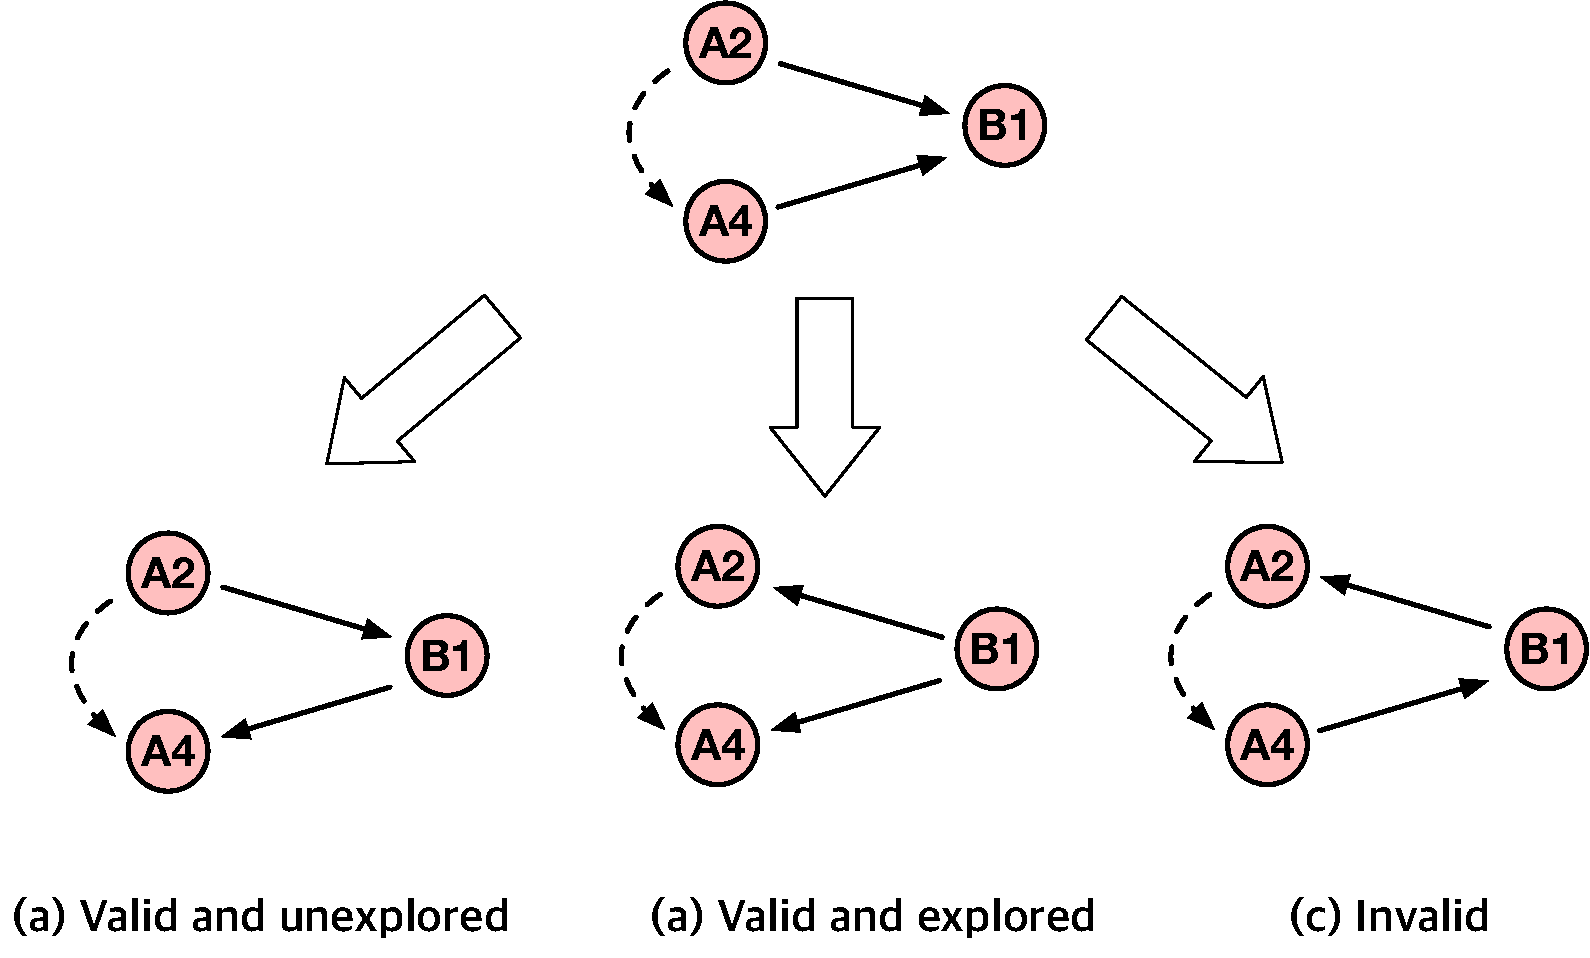
\includegraphics[width=0.7\linewidth]{fig/interleavingmutation.pdf}
  \caption{Example of interleaving segment mutation. In this example,
    (a) represents an interleaving segment graph of
    \autoref{fig:interleavingsegmentgraph} while (b) and (c) represent
    \textit{valid} mutated segments of (a). Whereas (d) is an
    \textit{invalid} mutated segment of (a) because it contains a
    loop.}
  \label{fig:interleavingmutation}
\end{figure}
%
\autoref{fig:interleavingmutation} illustrates how a fuzzer mutates a
segment graph.
%
For example, flipping ($\texttt{B1} \Rightarrow \texttt{A2}$) of
\autoref{fig:interleavingmutation}-(a) produces a segment graph
described in \autoref{fig:interleavingmutation}-(b), which describes
an interleaving different than \autoref{fig:interleavingmutation}-(a).
%
In \autoref{fig:interleavingmutation}-(a), \texttt{B1} is executed
before \texttt{A2} (\ie, $\texttt{B1} \Rightarrow \texttt{A2}$), while
in \autoref{fig:interleavingmutation}-(b), \texttt{A2} is executed
before \texttt{B1} (\ie, $\texttt{A2} \Rightarrow \texttt{B1}$).
%
Likewise, flipping both of $(\texttt{B1} \Rightarrow \texttt{A2})$ and
$(\texttt{B1} \Rightarrow \texttt{A4})$ generates another segment
graph of \autoref{fig:interleavingmutation}-(c), which also represents
another interleaving.
%
Besides (b) and (c), however, flipping only
$(\texttt{B1} \Rightarrow \texttt{A4})$ of
\autoref{fig:interleavingmutation}-(a) generates an \textit{invalid}
segment graph described in \autoref{fig:interleavingmutation}-(d),
which contains a loop
$\texttt{B1} \Rightarrow \texttt{A2} \Rightarrow \texttt{A4}
\Rightarrow \texttt{B1}$.
%
Since edges represent execution orderings, a loop in a segment graph
indicates a contradiction on the execution order, stating that any
vertex on the loop should be executed before itself. Therefore, when a
mutated segment contains a loop, a fuzzer discards the segment.
%


In this way, a fuzzer generates mutated segments of all $g_i \in G$,
while excluding 1) invalid segments (\ie, ones that contain a loop),
and 2) explored segments (\ie, ones that their hash values are
recorded in the hash table).
%
As a result, a fuzzer forms a set of \textit{unexplored} mutated
segments $G_{mutated}$, and utilizes $G_{mutated}$ to determine how to
schedule instructions in future iterations.





\PP{Recomposing interleaving segments into whole interleaving}
%
One could select one mutated segment in $G_{mutated}$ and run an input
while enforcing interleavings describing in the mutated segment.
%
However, it might require many executions because the size of
$G_{mutated}$ could be large.
%
Instead, we select multiple mutated segments in $G_{mutated}$, and
\textit{recompose} them into whole interleaving to run selected
mutated segments at one.

% choose a more efficient way. We \textit{recompose} a new
% thread interleaving from $G^*_{mutated} \subseteq G_{mutated}$, and by
% running the recomposed thread interleaving, we test multiple unexlored
% segment mutations in $G^*_{mutated}$ at once.


\begin{figure}[t]
  \centering
  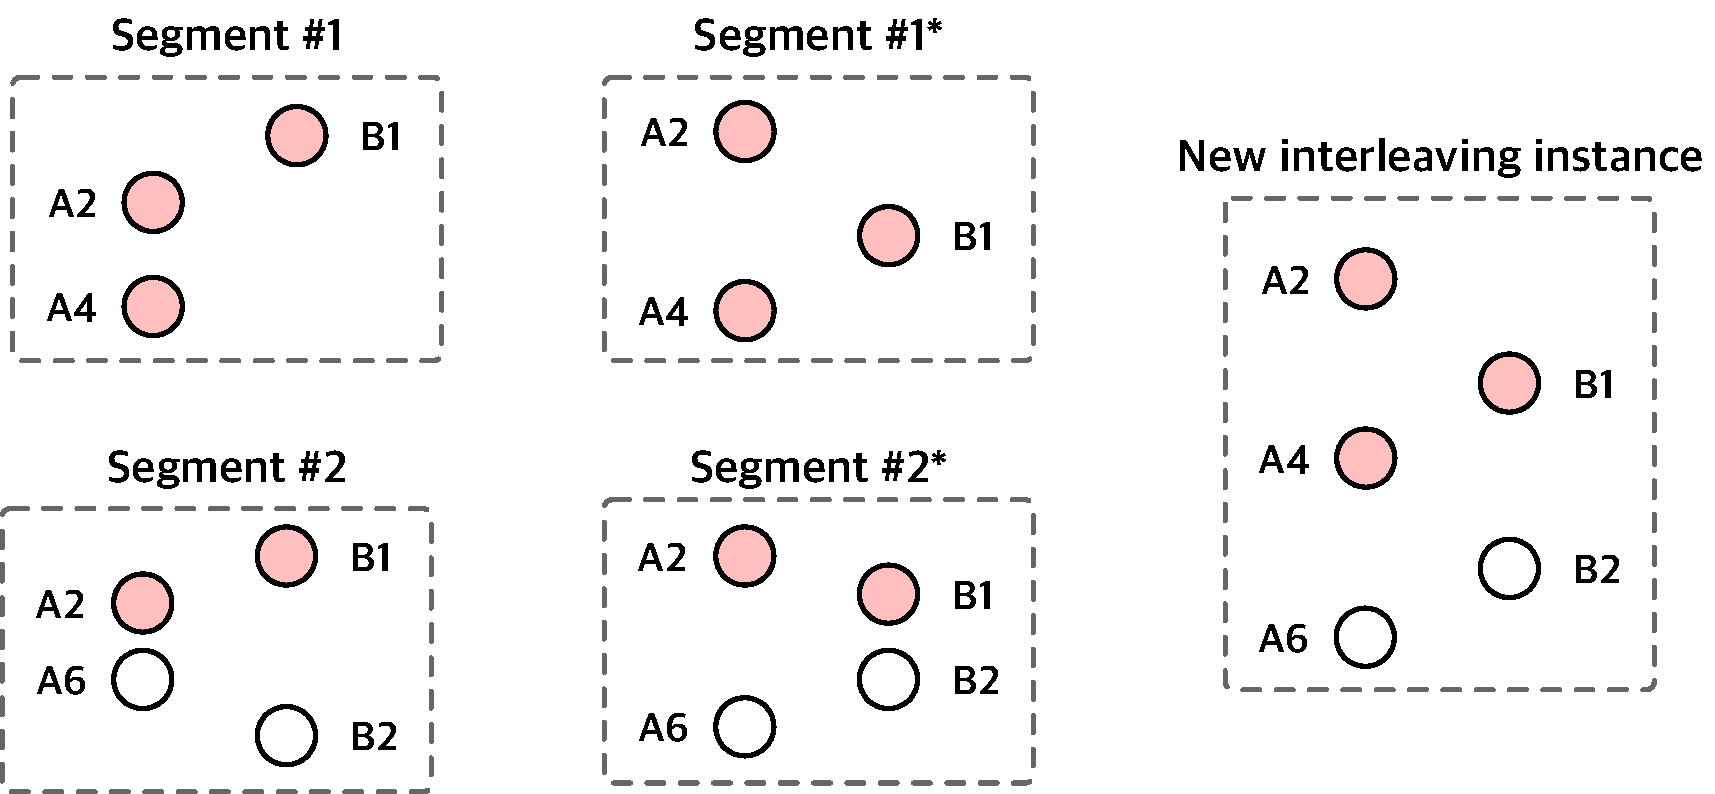
\includegraphics[width=0.85\linewidth]{fig/hint.pdf}
  \caption{Example of recomposing mutated segments into whole
    interleaving. (a) represents mutated segments, (b) represents a
    graph combining the two mutated segments, and (c) represents whole
    interleaving to test \texttt{Segment \#1*} and \texttt{Segment
      \#2*}}
  \label{fig:hint}
\end{figure}



\autoref{fig:hint} demonstrates an idea of how we recompose into whole
interleaving. Suppose we have two mutated segments \texttt{Segment
  \#1*} and \texttt{Segment \#2*} described in \autoref{fig:hint}-(a).
%
We can then draw a graph which contains all vertices and all edges
from \texttt{Segment \#1*} and \texttt{Segment \#2*} as described in
\autoref{fig:hint}-(b).
%
It is worth noting that \autoref{fig:hint}-(b) contains five vertices
and six edges, which is a superset of vertices and edges from
\texttt{Segment \#1*} and \texttt{Segment \#2*} respectively.
%
Therefore, when we execute a thread interleaving corresponding to this
graph, we can test both \texttt{Segment \#1*} and \texttt{Segment
  \#2*} at once (\autoref{fig:hint}-(c)).



When recomposing a thread interleaving, one important constraint is
that it should not contain a loop (\ie, \autoref{fig:hint}-(b) should
not contain a loop). Otherwise, a contradiction on the execution order
arises similar with an invalid mutation (\ie, an instruction should be
executed before itself).
%
To select a subset $G^*_{mutated}$ without making a loop, we start
with an empty set of $G^*_{mutated}$. Then, we iterate over mutations
in $g^* \in G_{mutated}$. With $g^*$, we determine adding edges in
$g^*$ into $G^*_{mutated}$ forms a loop or not. If it does not form a
loop, we add the segment graph into $G^*_{mutated}$.
%
After iterating all mutated segment graphs in $G_{mutated}$,
$G^*_{mutated}$ does not contain a loop. The fuzzer then excludes
selected segment graphs from the set of all mutated segment graphs
(\ie, $G_{mutated} = G_{mutated} \setminus G^*_{mutated}$), and
generates scheduling points to explore $G^*_{mutated}$.












\PP{Generating scheduling points}
%
Once $G^{*}_{mutated}$ is given, scheduling points can be easily
generated by conducting a topological sort~\cite{topologicalsort}.
%
Since an imaginary interleaving graph is acyclic, a topological sort
always returns a sequence of vertices (\ie, instructions) that does
not violate a program order.
%
It is well known that the time complexity of a topological sort is
$O(V+E)$. Considering that the graph is sparse, $E$ is a small value
so the time complexity can be asymptotically considered as $O(V)$.
%
In this sequence, scheduling points are just instructions that the
preemption should happen; \ie, the next instruction is executed by a
different thread.




%%% Local Variables:
%%% mode: latex
%%% TeX-master: "p"
%%% End:
